%!TEX TS-program = xelatex 
%!TEX encoding = UTF-8 Unicode

% Modify the following line to match your school
% Available options include `Harvard`, `Princeton`, and `NYU`.
\documentclass[School=NYU, 12pt]{Dissertate}

\begin{document}

\newcommand\blankpage{%
    \null
    \thispagestyle{empty}%
    %\addtocounter{page}{-2}%
    \newpage}

% Aman : The default name was ``Listing of figures"
\renewcommand{\listfigurename}{List of Figures}


\setmainfont{Times New Roman}
% the front matter
% Some details about the dissertation.
\title{Disentangling waves and vortices from limited observations}
\author{Han Wang}
\advisor{Dr. Oliver B{\"u}hler}

% ... about the degree.
\degree{Doctor of Philosophy}
\field{Mathematics & Atmosphere Ocean Sciences}
\degreeyear{2020}
\degreemonth{September}
\department{Department of Mathematics}


% ... about the candidate's previous degrees.
%\pdOneName{B.S.}
%\pdOneSchool{Boston University}
%\pdOneYear{2018}

%\pdTwoName{M.A.}
%\pdTwoSchool{Monster's University}
%\pdTwoYear{2021}
\maketitle

\pagenumbering{roman}

\begin{flushright}
\vspace{-20pt}
\rule{2.5in}{.4pt}\\
Oliver B{\"u}hler
\end{flushright}

%\setmainfont{Times New Roman}

% begin Aman : 
\setlength{\parindent}{0pt}

\copyrightpage
\dedicationpage
%\poem
%\afterpage{\blankpage}
\acknowledgments
\abstractpage
\tableofcontents
%\authorlist
%\cleardoublepage
%\addcontentsline{toc}{chapter}{\listtablename}
%\listoftables
\cleardoublepage
\addcontentsline{toc}{chapter}{\listfigurename}
\listoffigures


%\doublespacing

%\usepackage{fontspec}
%\setmainfont{Arial}

\justify
%\modulolinenumbers[2]  % to change the module of line numbers. Default 5 
% end Aman : 

\renewcommand\linenumberfont{\footnotesize}
% include each chapter...
%setcounter{chapter}{-1}  % start chapter numbering at 0
%\begin{linenumbers}

% Han, I am commenting this - so that you can compile this out of the box
\chapter{Introduction}
\label{introduction}
\pagenumbering{arabic}%added by Han
Write Introduction here
\chapter{Anisotropic Statistics of Lagrangian Structure Functions and Helmholtz Decomposition}
Write chapter content here
\chapter{Ageostrophic corrections for power spectra and wave--vortex decomposition} 
Write chapter content here
%\chapter{\rev{Concluding comments}}

Write chapter content here

%\end{linenumbers}{}

%\begin{appendices}
%    \include{chapters/appendixA}
%\end{appendices}

\singlespacing

% the back matter
\cleardoublepage
\addcontentsline{toc}{chapter}{References}

\bibliography{references}
\bibliographystyle{apalike} % amc is another option, but uses numbers

%\bibliographystyle{apalike2} % default

%\newpage

% If you do want an image in the colophon:
\begin{figure}
  \vspace{50pt}
  \centering
    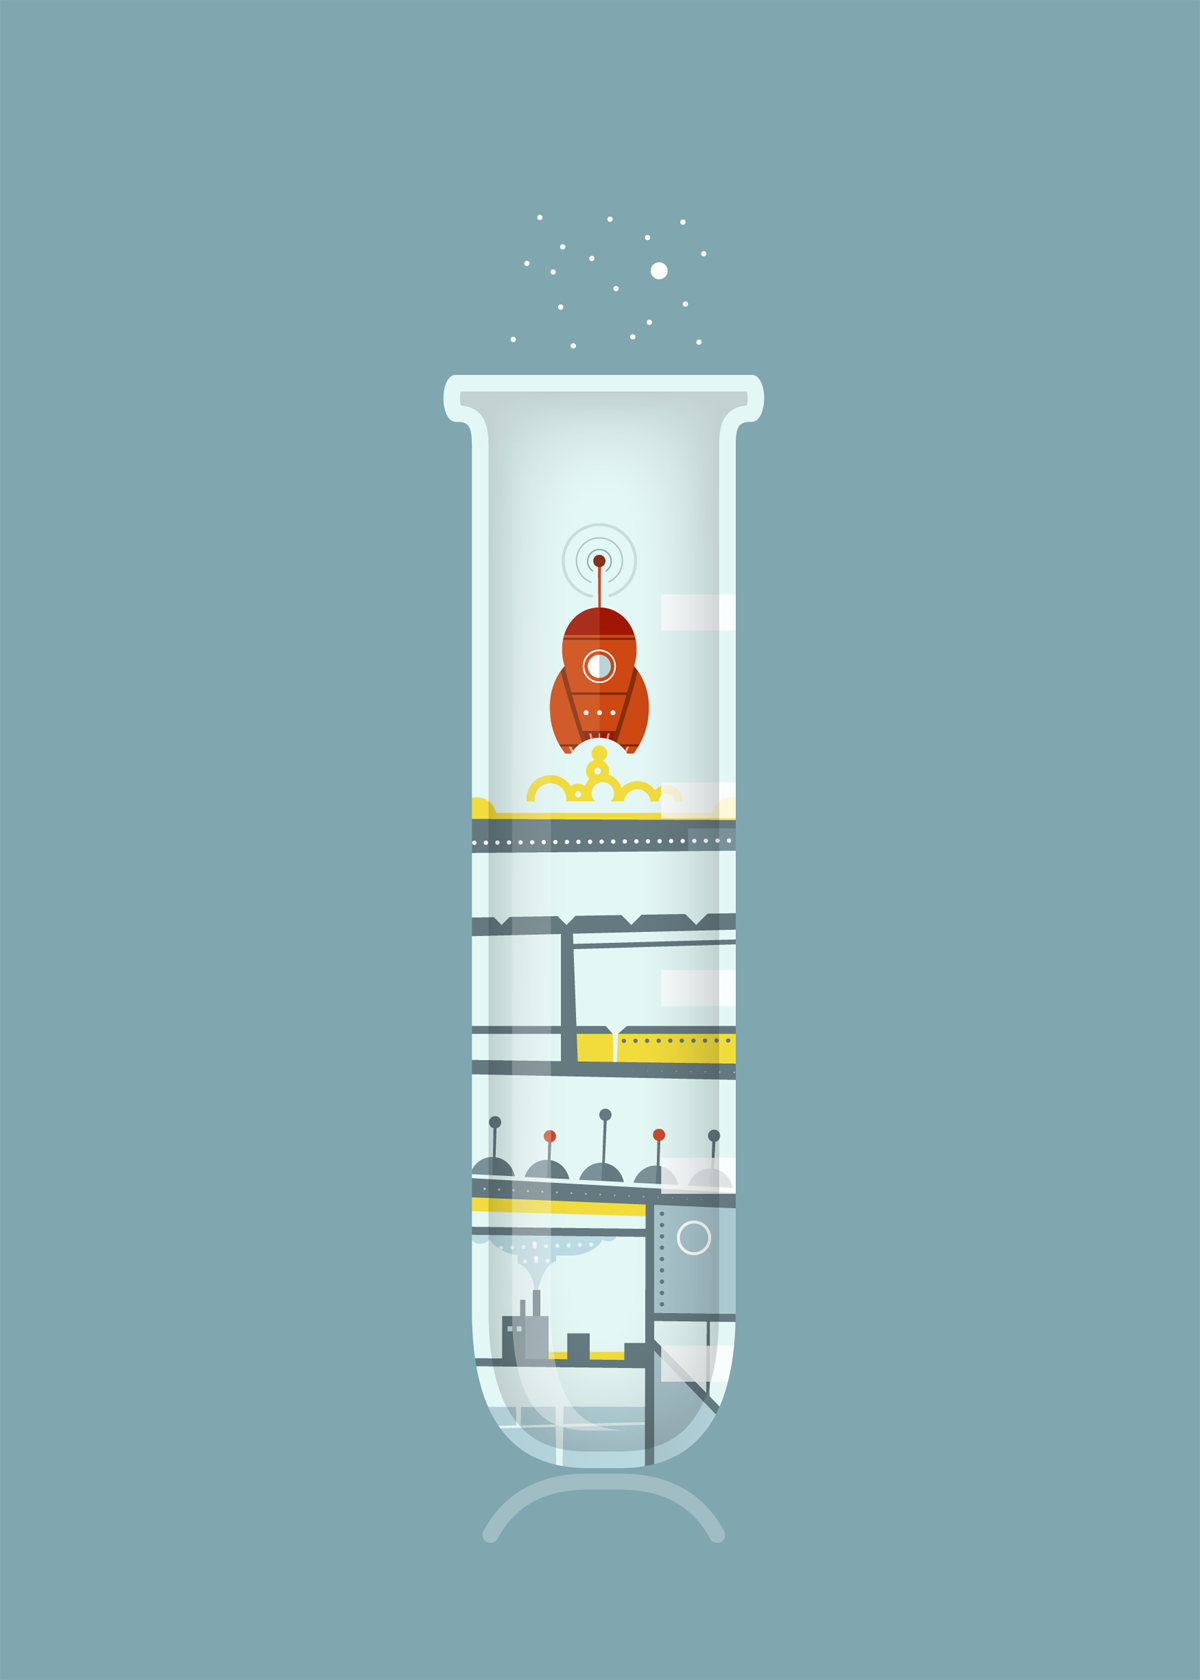
\includegraphics[width=0.51\textwidth]{endmatter/colophon.png}
\end{figure}

% If you don't want an image in the colophon:
% \vspace*{200pt}

\begin{center}
\parbox{200pt}{\lettrine[lines=3,slope=-2pt,nindent=-4pt]{\textcolor{SchoolColor}{T}}{his thesis was typeset} using \LaTeX, originally developed by Leslie Lamport and based on Donald Knuth's \TeX. The body text is set in 11 point Egenolff-Berner Garamond, a revival of Claude Garamont's humanist typeface. The above illustration, ``Science Experiment 02'', was created by Ben Schlitter and released under \href{http://creativecommons.org/licenses/by-nc-nd/3.0/}{\textsc{cc by-nc-nd 3.0}}. A template that can be used to format a PhD thesis with this look and feel has been released under the permissive \textsc{mit} (\textsc{x}11) license, and can be found online at \href{https://github.com/suchow/Dissertate}{github.com/suchow/Dissertate} or from its author, Jordan Suchow, at \href{mailto:suchow@post.harvard.edu}{suchow@post.harvard.edu}.}
\end{center}

\end{document}